\documentclass[oneside,english]{amsart}
\usepackage{bbold}
\usepackage[T1]{fontenc}
\usepackage{inputenc}
\setlength{\parskip}{\smallskipamount}
\setlength{\parindent}{0pt}
\usepackage{amstext}
\usepackage{amsthm}
\usepackage{amsmath}
\usepackage{amssymb}
\usepackage{graphicx}
\usepackage{multirow}
\usepackage{subcaption}
\usepackage{wasysym}


\makeatletter
\numberwithin{equation}{section}
\numberwithin{figure}{section}
\theoremstyle{plain}
\newtheorem{thm}{\protect\theoremname}
\theoremstyle{definition}
\newtheorem{defn}[thm]{\protect\definitionname}
\theoremstyle{plain}
\newtheorem{prop}[thm]{\protect\propositionname}
\theoremstyle{remark}
\newtheorem{rem}[thm]{\protect\remarkname}
\theoremstyle{plain}
\newtheorem{lem}[thm]{\protect\lemmaname}
\theoremstyle{definition}
\newtheorem{example}[thm]{\protect\examplename}
\newtheorem{cor}[thm]{\protect\corollaryname}
\theoremstyle{definition}

\makeatother

\usepackage{babel}
\providecommand{\definitionname}{Definition}
\providecommand{\lemmaname}{Lemma}
\providecommand{\propositionname}{Proposition}
\providecommand{\remarkname}{Remark}
\providecommand{\theoremname}{Theorem}
\providecommand{\examplename}{Example}
\providecommand{\corollaryname}{Corollary}

\begin{document}
\title{Tropical Support Vector Machines}
\author{Samuel Boïté, Théo Molfessis \\ Supervised by Xavier Allamigeon, Stéphane Gaubert}
\maketitle

\begin{abstract}
    We develop new algorithms around tropical support vector machines (SVMs) for binary and multi-classification. We explore the use of tropical hyperplanes to partition tropical space, laying the groundwork for our classification approach. We address the challenge of separating overlapping data in tropical space, proposing a method to measure and handle data overlap using non-expansive Shapley operators and a Krasnoselskii-Mann iteration scheme. For separable data, we extend our method to determine hard-margin tropical hyperplanes, ensuring maximal separation. This is further applied to multi-classification scenarios, providing conditions for tropical separability and demonstrating margin optimality. Additionally, the tropical kernel trick is explored as a means to embed data into a higher-dimensional tropical space, transforming decision boundaries into tropical polynomials. This approach is empirically tested on several classic datasets. Finally, we show that tropical hyperplanes emerge as limiting cases of classical hyperplanes on logarithmic paper, making our approach more stable numerically.
\end{abstract}

\section{Introduction}

% Add an introduction that explains the relevance of the topic

The tropical semifield $\mathbb{R}_{\max}$ is the set of real numbers,
completed by $-\infty$ and equipped with the addition $a\oplus b=\max(a,b)$
and the multiplication $a\odot b=a+b$.
\begin{defn}
A \emph{tropical hyperplane of apex $a\in\mathbb{R}_{\text{max}}^{d}$
}splits $\mathbb{R}_{\max}^{d}$ depending on where $(x-a)$ reaches
its maximum coordinate: 
\[
H_{a}:=\left\{ x\in\mathbb{R}_{\max}^{d},\quad(x-a)\,\,\text{reaches its max coordinate at least twice}\right\} .
\]

It hence partitions the space between $d$ different \emph{tropical
sectors}. A \emph{tropical halfspace} of configuration $I\subset[d]$
is the union of tropical sectors specified in $I$.

Let $n\in[d]$. We define the \emph{tropical parametrized hyperplane} of configuration
$\sigma=\{I^{1},\ldots,I^{n}\}$, where $I^k \cap I^\ell = \emptyset$ for $k\ne l$, as:
\[
H_{a}^{\sigma}:=\left\{ x\in\mathbb{R}_{\max}^{d},\quad\exists k\ne\ell,\quad(x-a)\,\,\text{reaches its max coordinate in}\,I^{k}\,\text{and}\,I^{\ell}\right\} .
\]
When $n=2$, we talk about \emph{tropical signed hyperplanes}. Generally,
a tropical parametrized hyperplane is the union of tropical signed
hyperplanes defined by all pairs of sectors.
\end{defn}

\begin{defn}
We define the \emph{tropical span} of a finite set of points $X=(x_{1},\ldots,x_{p})\in\mathbb{R}_{\max}^{d\times p}$
as the set of tropical linear combinations of these points.
\[
\text{Span}(X):=\left\{ \lambda X:=\max_{i\in[p]}\left(x_{i}+\lambda_{i}\right),\quad\lambda\in\mathbb{R}^{p}\right\} .
\]
Given the tropical convexity of these, these spans are often called
\emph{tropically convex hulls}, meaning the smallest tropically convex
sets containing them. 
\end{defn}

\textbf{The tropical classification problem. }We want to separate
$n\in[d]$ classes of $d$-dimensional data points $X^{1},\ldots,X^{n}$
using a tropical parametrized hyperplane of configuration $\sigma$.
In the binary setting, we note the classes $X^{\pm}$ consisting of
the points with positive (resp. negative) labels. Separating them
tropically amounts to separating their spans, noted $V^{1},\ldots,V^{n}$
or $V^{\pm}$ in the binary setting.
\begin{defn}
For all $u\in\mathbb{R}_{\max}^{d}$, we define the \emph{tropical
norm} of $u$ as the largest difference between two of its coordinates:
\[
\lVert u\rVert:=\max u-\min u.
\]
The \emph{tropical distance} between $u$ and $v$ in $\mathbb{R}_{\max}^{d}$
is then deduced as: 
\[
d(u,v):=\lVert u-v\rVert.
\]
\end{defn}

\begin{defn}
$H_{a}^{\sigma}$ is said to \emph{separate point clouds $(X^{k})_{k\in[n]}$
with a margin of at least} $\nu\ge0$ when for all $x^{k}\in X^{k}$,
$k\in[n]$:
\begin{enumerate}
\item $x^{k}$ is on the correct side of the hyperplane $H_{u}^{\sigma}$,
that is:
\[
\underset{i\in[d]}{\arg\max}\, x_{i}^{k}\in I^{k}.
\]
\item Distance from $H_{a}^{\sigma}$ to $x^{k}$ is at least $\nu$:
\[
d(H_{a}^{\sigma},x^{k})=\max(x^{k}-a)-\max_{\bigsqcup_{\ell \ne k} I^\ell}(x^{k}-a)\ge\nu.
\]
\end{enumerate}
When $\nu$ is maximal in the previous definition, we say that $H_{a}^{\sigma}$
\emph{separates with a margin of} $\nu$. When $\nu$ is zero, we
say that $H_{u}^{\sigma}$ \emph{separates} $(X^{k})_{k\in[n]}$. 
\end{defn}


\begin{figure}[!h]
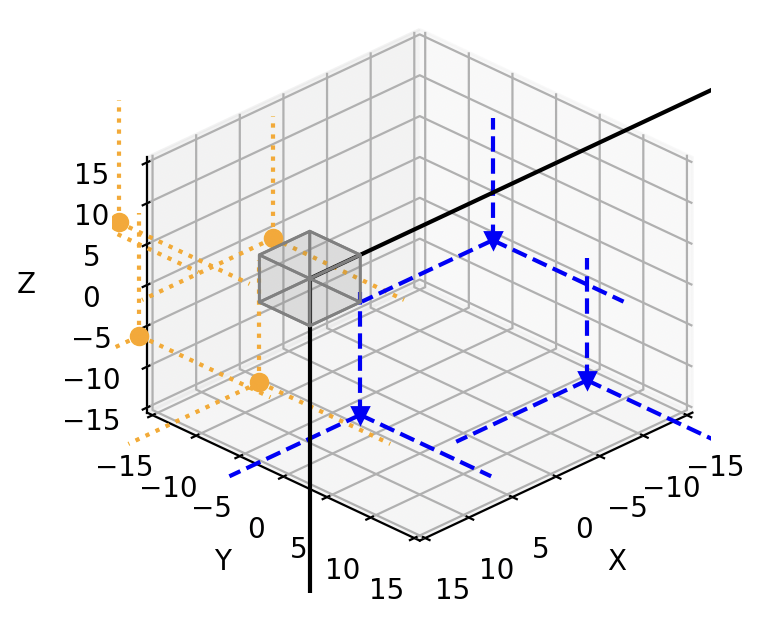
\includegraphics[scale=0.8]{fig/illustration.png} \caption{Tropical Binary Classification Example}
\end{figure}


\section{Tropical Binary Classification}

For the moment, let's confine ourselves to binary classification.

\subsection{Tropical projections and Shapley operators}

In this section, we see that Shapley operators are the appropriate
framework for describing and tropically separating finite point clouds,
in particular but not exclusively.
\begin{defn}
A \emph{Shapley operator} on $\mathbb{R}_{\max}$ is a map $T:\mathbb{R}_{\max}^{d}\longrightarrow\mathbb{R}_{\max}^{p}$
such that $T$ is non-decreasing and that for all $x\in\mathbb{R}_{\max}^{n}$
and $\lambda\in\mathbb{R}_{\max}$, $T(\lambda+x)=\lambda+T(x)$.

$T$ is said to be \emph{non-expansive }if it is $1$-Lipschitz. 
\end{defn}

\begin{defn}
A Shapley operator $T$ is said to be \emph{diagonal free} when $T_{i}(x)$
is independent of $x_{i}$ for all $i\in[n]$. That is, when for all
$i\in[n]$, and for all $x,y\in\mathbb{R}_{\max}$ such that $x_{j}=y_{j}$
for all $j\neq i$, we have $T_{i}(x)=T_{i}(y)$. 
\end{defn}

\begin{defn}
Let $V$ a tropically convex, compact and nonempty subset of $\mathbb{R}_{\max}^{d}$.
We define the \emph{projection} of $x$ on $V$ as: 
\[
P_{V}(x):=\max\{y\in V,\quad y\le x\}.
\]
When $V=\text{Span}(X)$ with $X$ in $\mathbb{R}_{\max}^{d\times p}$,
we will write the projection as $P_{X}$.
\end{defn}

\begin{prop}
\label{prop:(Nondecreasing)}Let $X\in\mathbb{R}_{\max}^{d\times p}$.
$P_{X}$ is nondecreasing and for $x\in\mathbb{R}_{\text{max}}^{d}$,
$P_{X}(x)\le x$. Moreover, we know from Maclagan et al. \cite{Maclagan2015}
that:
\[
\forall i\in[p],\quad P_{X}(x)=\max_{j\in[p]}\left\{ X_{ij}+\min_{k\in[d]}(-X_{kj}+x_{k})\right\} .
\]
\end{prop}

\begin{rem}
Tropical projections, and Shapley operators in general, are closely
tied to mean payoff games: for instance, let's define $T$ as
\[
\forall i\in[n],\quad T_{i}(x)=\max_{j\in[p]}\left\{ A_{ji}+\min_{k\in[n]}(-B_{jk}+x_{k})\right\} .
\]
Here, $T_{i}(0)$ is the payoff, recieved by player MIN,
of one round of a game with perfect information, where player
MAX starts from their state $i$, transitions to their opponent MIN's
state $j$ by receiving $A_{ji}$, who in turn chooses a MAX state
$k$ by recieving $B_{jk}$.

Therefore, $(T^{m}(0))_{i}$ is the \emph{value} of such a game after
$m$ consecutive rounds, having started in the MIN state $i$. The\emph{
escape rate }of the game defined by $T$ is defined by: 
\[
\chi_{T}:=\lim_{m\rightarrow+\infty}\frac{T^{m}(0)}{m}.
\]
It is well known that this limit does exist and coincides with the
\emph{mean payoff} of the game \cite{Allamigeon2018}. Under certain
conditions, $\chi_{T}$ is the unique eigenvalue of the Shapley operator
$T$. 
\end{rem}

\begin{defn}
Let $T$ be a non-expansive Shapley operator. We define
\[
\text{\ensuremath{\mathcal{S}(T)}}=\{x\in\mathbb{R}^{d},\quad x\le T(x)\}.
\]
\end{defn}

\begin{prop}
Let $P_{V}$ be the tropical projection on $V$. Then:
\[
\ensuremath{\mathcal{S}(P_{V})=V}.
\]
\end{prop}

\begin{proof}
As $P_{V}(x)\le x$ for any $x$, $x\le P_{V}(x)$ (i.e $x\in\mathcal{S}(T)$)
is equivalent to $x=P(x)$ (i.e $x\in V$).
\end{proof}
\begin{rem}
Operator $P$ can be slightly tweaked to make it \emph{diagonal-free}
(DF), a good property that will be of interest to us in the future.
In the modified game, the MAX player is prevented from replying to
his opponent eye-for-an-eye:
\[
\left[P_{\text{DF}}(x)\right]_{i}:=\max_{j\in[p]}\left\{ X_{ij}+\min_{k\ne i}(-X_{kj}+x_{k})\right\} .
\]
Beware, this is not a projector anymore!
\end{rem}

\begin{prop}
$P_{\text{DF}}$ is a diagonal-free Shapley map that equivalently
describes $X$. 
\end{prop}

\begin{proof}
$P_{\text{DF}}$ is a Shapley operator for the same reasons $P$ is,
and its formula directly proves it is diagonal free. We then note
that $P\leq P_{\text{DF}},$ therefore $\mathcal{S}(F)\subset\mathcal{S}(F_{\text{DF}}).$
Let $x\in\mathcal{S}(P_{\text{DF}})$, and $i\in[n]$. There exists
$j\in[p]$ such that
\[
x_{i}\leq-X_{ij}+\min_{k\ne i}(-X_{kj}+x_{k}).
\]
That inequality holds for $k=i$, hence $x_{i}\leq P_{i}(x)$ and
finally $\mathcal{S}(P)=\mathcal{S}(P_{\text{DF}}).$
\end{proof}

\subsection{Separating finite overlapping data}

Assuming that the data overlap, we want to find a way to transform
them slightly to make them separable by a tropical hyperplane. This
would give us a measure of their non-separability.

\subsubsection{Measuring data overlap}

We want a simple criteria for computing the size of the intersection
between convex hulls.
\begin{lem}
Let $(T^{i})_{i\in[n]}$ be non-expansive Shapley operators. We have:
\[
\bigcap_{i\in[n]}\mathcal{S}(T^{i})=\mathcal{S}\left(\bigwedge_{i\in[n]}T^{i}\right),
\]
\end{lem}

According to \cite{AKIAN2012}, when we have non-expansive Shapley
operators, the notions of Collatz-Wielandt numbers, spectral radus
and game value are identical . We can then state the following theorem: 
\begin{thm}
(Allamigeon, Gaubert et al. \cite{Allamigeon2018}) $V$ contains
a Hilbert ball of positive radius if and only if the spectral radius
of $F$, defined as 
\[
\rho(T)=\sup\{\mu\in\mathbb{R},\quad\exists z\in\mathbb{R}^{d},\quad T(z)=\mu+z\},
\]
is strictly positive. In this case, $\rho(F)$ is the inner radius
$\text{inrad}(V^{+}\cap V^{-})$, i.e supremum of the radii of the
Hilbert balls contained in it. 
\end{thm}

We can then apply the following Krasnoselskii-Mann algorithm to compute
the eigenpair in pseudo-polynomial time. Given an initial point $a^{0}$,
we iteratively compute: 
\[
\begin{cases}
z^{k+1} & =\frac{a^{k}+T(a^{k})}{2}\\
a^{k+1} & =z^{k+1}-\max_{i\in[d]}z_{i}^{k+1}\cdot\textbf{1}_{d}
\end{cases}
\]

The following convergence theorem follows from \cite{Cominetti2013}:
\begin{cor}
As $T$ is a non-expansive Shapley operator, the Krasnoselskii-Mann
algorithm converges in pseudo-polynomial time. 
\end{cor}

The eigenpair we search is $\left(a^{\infty},2\cdot\max_{i\in[d]}z_{i}^{\infty}\right)$.

\subsubsection{Separating two classes of data}

We place ourselves back in the binary classification setting. We have
described the corresponding Shapley operators corresponding to our
classes as diagonal-free maps. We now define a process for separating
overlapping data. Assuming $V^{+}\cap V^{-}\ne\emptyset$, let $\left(a,\lambda\right)$
be the eigenpair of $T:=T^{+}\wedge T^{-}$ approximated by the previously
described iteration algorithm. 
\begin{prop}
We project all points of $X^{\pm}$ located at a distance less than
$\lambda$ from $H_{a}$, onto $H_{a}$. Then the intersection
of new convex hulls $W^{\pm}$ is of empty interior. 
\end{prop}

\begin{proof}
Let's denote $X$ the cloud consisting of all points (regardless of
sign), and for $x_{j}\in X$, we note $y_{j}$ its sign, $s_{j}$
its sector and $d_{j}$ the second argmax of $(x_{j}-a)$. For each
point $x_{j}=X_{\cdot j}\in X$ at distance less than $\lambda$ of
$H_{a}$, the transformation consists in setting
\[
W_{kj}:=\begin{cases}
X_{kj} & \text{if \ensuremath{k\ne s_{j}}}\\
X_{s_{j}j}-d(x_{j},H_{a}) & \text{at \ensuremath{s_{j}}}
\end{cases}
\]
so that $w_{j}$ is projected on the hyperplane. As $T^{\pm}$ is
non-expansive and diagonal-free, let's remark that for $x^{\pm}\in V^{\pm}$:
\[
x_{i}^{\pm}\le T^{\pm}(x^{\pm})_{i}=\left(T^{\pm}(x^{\pm})-T^{\pm}(a)\right)_{i}+T^{\pm}(a)_{i},
\]
hence 
\begin{equation}
x_{i}^{\pm}\le\max(x^{\pm}-a)_{\ne i}+T^{\pm}(a)_{i}.\label{eq31}
\end{equation}
Let $i\in[d]$. If $x_{j}\in X$ is not in the $i$-th sector, then
for $k$ different from the sector of $x_{j}$, by definition:
\[
(w_{j}-a)_{k}\le(x_{j}-a)_{d_{j}}\le(w_{j}-a)_{s_{j}},
\]
hence
\[
W_{ij}-\max_{k\ne i}\left(W_{kj}-a_{k}\right)\le a_{i}.
\]
Otherwise, $x_{j}$ is in the $i$-th sector and:
\[
\max_{k\ne i}\left(W_{kj}-a_{k}\right)=X_{d_{j}j}-a_{d_{j}},
\]
thus
\[
W_{ij}-\max_{\ne i}\left(w_{j}-a\right)=\left(w_{j}-a\right)_{s_{j}}-\left(x_{j}-a\right)_{d_{j}}+a_{s_{j}}\ge a_{s_{j}}=a_{i},
\]
with equality iff $d(x_{j},H_{a})\leq\lambda$.

Suppose by symmetry that $T(a)_{i}=T^{+}(a)_{i}=\lambda+a_{i}.$ We
also have $T^{-}(a)_{i}\ge\lambda+a_{i}$. Then, using the proof of
Theorem 22 in \cite{Akian2021TropicalLR}, we know that there exists
$j^{+},j^{-}\in[p]$ such that $x_{j^{+}}\in X^+$ and $x_{j^{-}}\in X^-$ are in sector $i$,
with $x_{j^{+}}$ being at distance $\lambda$ from $H_{a}$ and $x_{j^{-}}$
at distance greater than $\lambda$. Therefore, $W_{ij^+}-\max_{\ne i}\left(w_{j^+}-a\right)=a_{i}$
and $W_{ij^-}-\max_{\ne i}\left(w_{j^-}-a\right)\geq a_{i}$. Moreover, for any $j$ such that $x_{j}\in X^+$ is in sector
$i$, eq. \ref{eq31} gives $d(x_{j},H_{a})\leq\lambda$.

Let $Q^{\pm}$ be the \emph{diagonal-free} projections over transformed
point clouds, and 

$Q=Q^{+}\wedge Q^{-}.$ We've just shown that 
$Q(a)_{i}=Q^{+}(a)_{i}=a_{i}$,
and finally $Q(a)=a$.


\end{proof}
\newpage
\begin{example}

Here is what the transformation yields with a toy inseparable dataset:

\begin{figure}[!h]
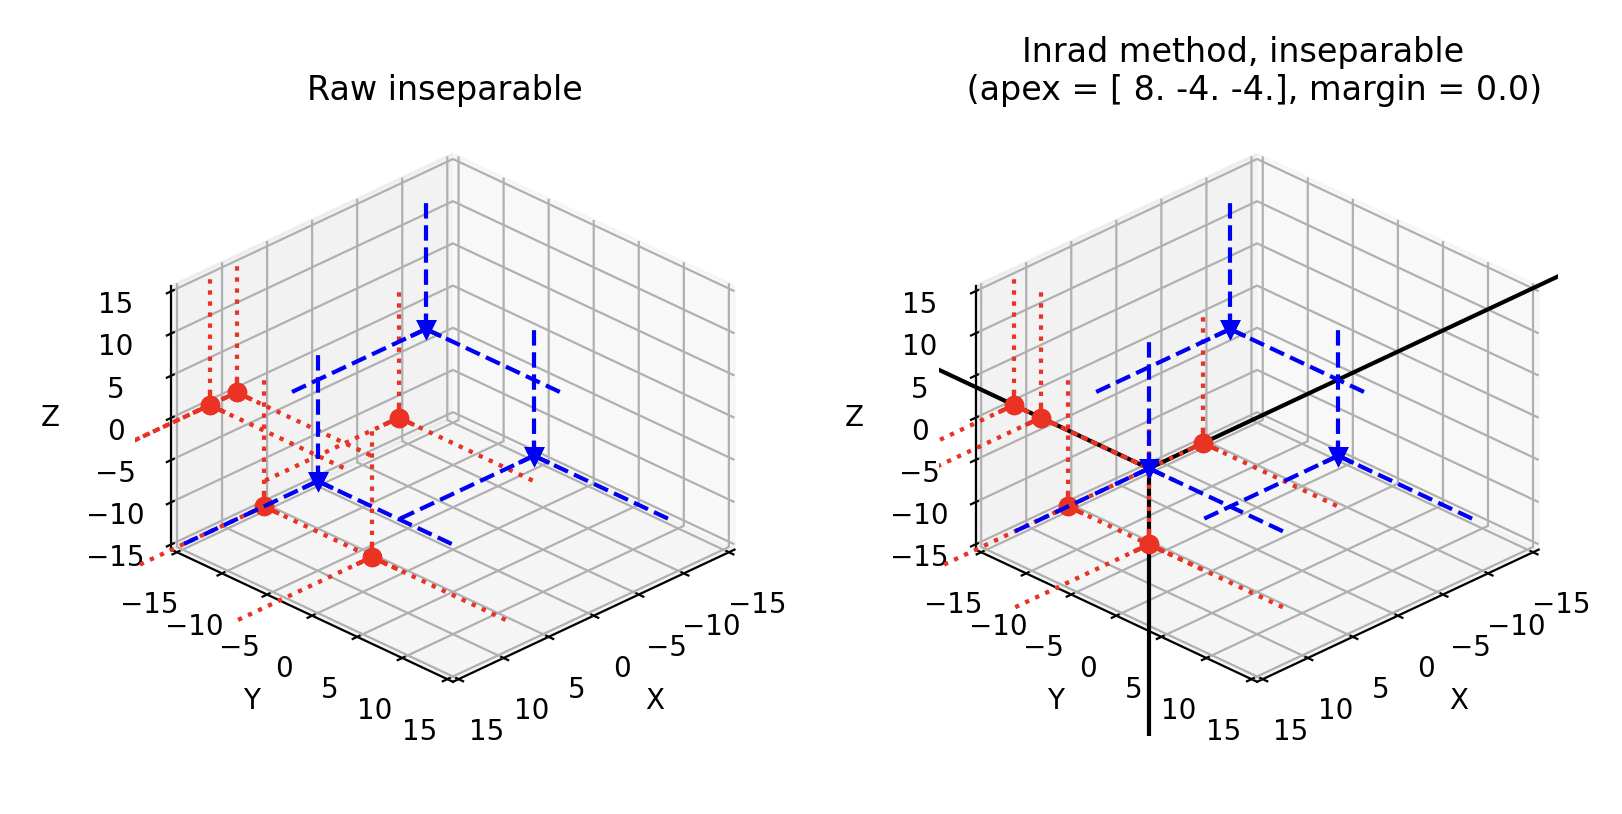
\includegraphics[scale=0.4]{fig/inseparable} \caption{Separating convex hulls}
\end{figure}
\end{example}

\begin{rem}
In order to strictly separate the sets, we would have to deal with
the branching points of null interior. 
\end{rem}

In pseudo-polynomial time, we are thus able to compute a distance
of our point clouds to separability. It gives a bound on the distance
under which some points have to be moved to separate hulls.

\subsection{Optimal hard-margin in the separable case}

Assuming that data is now separable, we prove that the previous method
can be extended to give us separating hyperplanes with maximal margin. 
\begin{rem}
When $V^{+}$ and $V^{-}$ are disjoint, the spectral radius $\lambda$
of $T$ is strictly negative. From \cite{AKIAN2021}, we may see $-\lambda$
as the eigenvalue an operator $T^{\text{dual}}$ in dual space, as
$T$ is itself a finitely-generated Shapley operator. This would give
us a complementary inner radius interpretation, and makes $H_{a}$
a great candidate in the separable case. 
\end{rem}

Let $(a,\lambda)$ the eigenpair of $T$ approximated by previous
algorithm, verifying $T(a)=\lambda+a$. Let's define the sectors:
\[
I^{\pm}:=\{i\in[d],\quad T^{\pm}(a)_{i}>\lambda+a_{i}\},
\]
and the corresponding configuration $\sigma=\{I^{\pm}\text{\}}.$
\begin{prop}
$H_{a}^{\sigma}$, given the sectors defined above, separates $V^{+}$
and $V^{-}$ with a margin of $-\lambda$. Moreover, this margin is
optimal in the case where $T^{\pm}$ are of the form $T^{\pm}(x)=P_{V^{\pm}}(x)=\sup_{v\in V^{\pm}}\left(v_{i}+\min(-v+x)\right),$
which is in particular the case when separating finite point clouds. 
\end{prop}

\begin{proof}
As $T^{\pm}$ is non-expansive, let's first remark that for $x^{\pm}\in V^{\pm}$:
\[
x_{i}^{\pm}\le T^{\pm}(x^{\pm})_{i}=\left(T^{\pm}(x^{\pm})-T^{\pm}(a)\right)_{i}+T^{\pm}(a)_{i},
\]
hence 
\begin{equation}
x_{i}^{\pm}\le\max(x^{\pm}-a)+T^{\pm}(a)_{i}.\label{eq41}
\end{equation}
For instance, let $i\in[d]\setminus I^{+}$. Then $T^{+}(a)_{i}=\lambda+a_{i}$,
so for $x^{+}\in V^{+}$, using equation \ref{eq41}:

\[
x_{i}^{+}-a_{i}\le\max(x^{+}-a)+\lambda.
\]

In particular, $x_{i}^{+}-a_{i}<\max(x^{+}-a)$ and any element of
$V^{+}$ can't belong to any of sectors in $[d]\setminus I^{+}$ with
respect to $H_{a}$, from which the sectors $I^{\pm}$ are well-defined.
Finally, 
\[
d(H_{a}^{I^{+}},x^{+})=\max(x^{+}-a)-\max(x^{+}-a)_{[d]\setminus I^{+}}\ge-\lambda,
\]
and the margin comes from the fact that this applies to any element
of $V^{+}$.

Let's finally prove that the margin is maximal in the case where $T^{\pm}$
are of the form $T^{\pm}(x)=P_{V^{\pm}}(x)=\sup_{v\in V^{\pm}}\left(v_{i}+\min(-v+x)\right).$
Let $i\in[d]\setminus I^{+}$. Then, for $\varepsilon>0$, we can
find $v\in V^{+}$ such that 
\[
T^{+}(a)_{i}-\varepsilon\le v_{i}-\max(v-a)\le T^{+}(a)_{i},
\]
giving us 
\[
\lambda-\varepsilon\le v_{i}-a_{i}-\max(v-a)\le\lambda.
\]
Maximizing over all $i\in[d]\setminus I^{+}$ yields that $v$ is
at most at distance $-\lambda+\varepsilon$ of $H_{a}^{I}$, hence
the optimality.
\end{proof}
\begin{example}
Here is what the algorithm gives with a toy separable dataset:

\begin{figure}[!h]
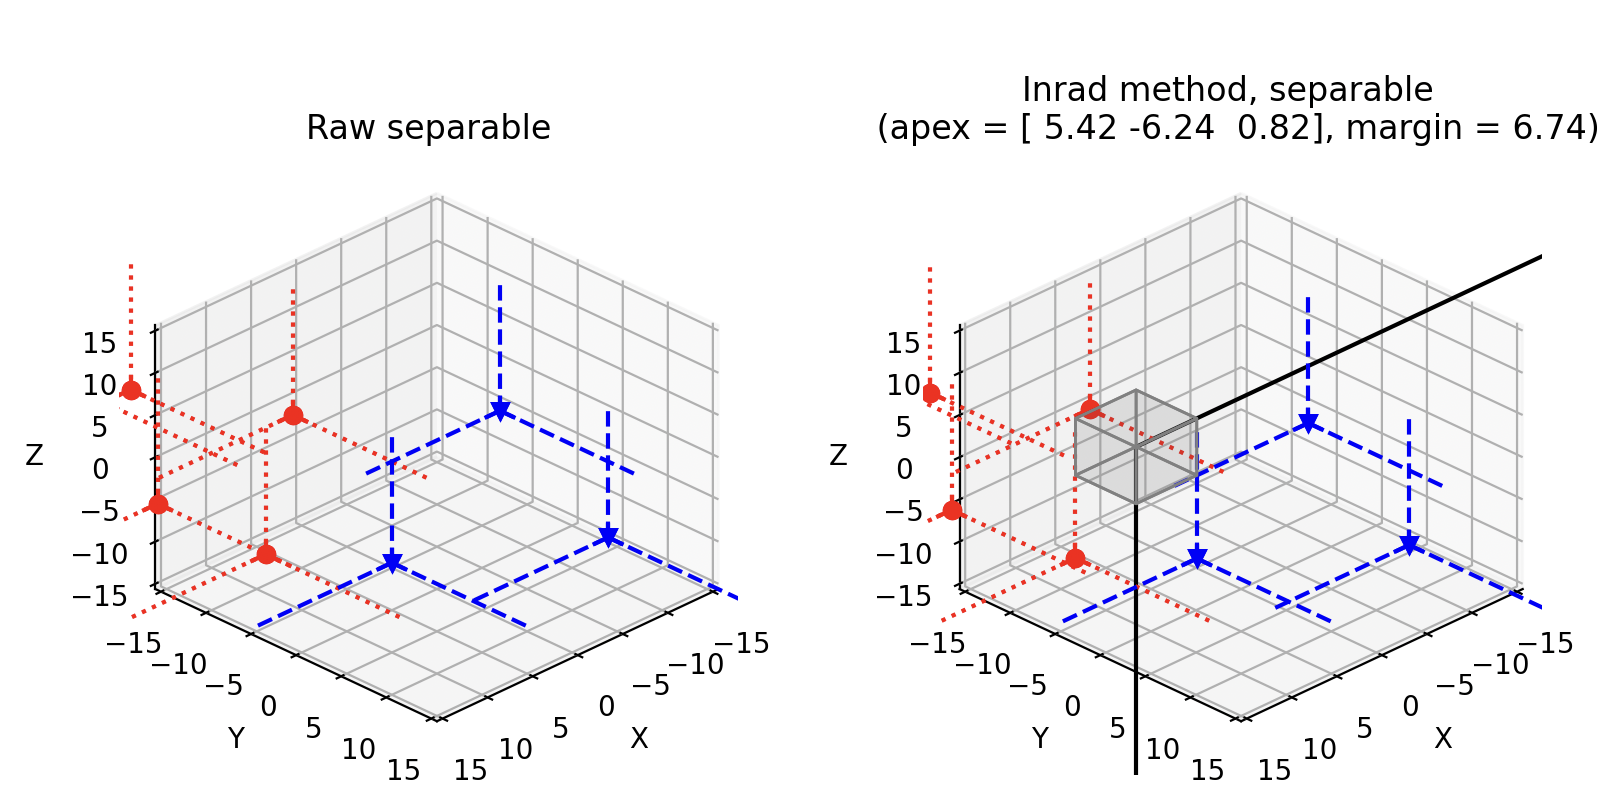
\includegraphics[scale=0.45]{fig/separable} \caption{Optimal-margin separable hyperplane}
\end{figure}
\end{example}


\section{Topics Being Explored}

\subsection{Hard-Margin Multi-Classification}

In this section, we consider convex hulls of point clouds of $n$
classes, noted $V^{k}$ for $k\in[n]$, and described by Shapley operators
$T^{k}$. We give a sufficient condition for these classes to be tropically
separable in their whole, meaning that there exists a tropical signed
hyperplane such that each $V^{k}$ belong to sectors of $I^{k}\subset[d]$
with $I^{k}\cap I^{l}=\emptyset$ for $k\ne l\in[n].$ We then adapt
the previous results to this case.

We now consider the Shapley operator :

\[
T:=\bigvee_{1\le k<l\le n}T^{k}\wedge T^{l}
\]

We remark that in the case $n=2$, $T$ is the same as previously
defined.

Let $(a,\lambda)$ the eigenpair of $T$ approximated by the Kranoselskii-Mann
algorithm, verifying $T(a)=\lambda+a$. Let's define the sectors:
\[
I^{k}:=\{i\in[d],\quad T^{k}(a)_{i}>\lambda+a_{i}\}.
\]

Given the definition of $T$, it is clear that $I^{k}\cap I^{l}=\emptyset$
for $k\ne l\in[n],$ and we have the following result :
\begin{prop}
If $\lambda<0$, the tropical parametrized hyperplane $H_{a}^{\sigma}$,
given the configuration $\sigma=\{I^{k}\}_{k\in[n]}$, separates $V^{k}$
and $V^{l}$ for all $k\ne l\in[n]$ with a margin of $-\lambda$.
Moreover, this margin is optimal in the case where all $T^{k}$ are
of the form
\[
T^{k}(x)=P_{V^{k}}(x)=\sup_{v\in V^{k}}\left(v_{i}+\min(-v+x)\right),
\]
 which is in particular the case when separating finite point clouds. 
\end{prop}

\begin{proof}
Let $k\in[n]$ and $i\in[d]\setminus I_{k}$. Using the same reasoning
as in the proof of Proposition $19$, we obtain that for all $x^{k}\in V^{k}$,
\[
d(H_{a}^{\sigma},x^{k})=\max(x^{k}-a)-\max(x^{k}-a)_{[d]\setminus I_{k}}\ge-\lambda,
\]
hence the margin. Let's now prove the optimality in the case where
all $T^{k}$ are of the form $T^{k}(x)=P_{V^{k}}(x)=\sup_{v\in V^{k}}\left(v_{i}+\min(-v+x)\right).$
For all $i\in[d]$, there are two distinct classes $k\ne l\in[n]$
such that $T^{k}(a)_{i}\wedge T^{l}(a)_{i}=\lambda+a_{i}$. As $I^{k}\cap I^{l}=\emptyset$,
we can suppose by symmetry that $i\in[d]\setminus I_{k}.$ Then using
the same argument as in the proof of optimality in Proposition $19$,
we know that for all $\varepsilon>0$ there is a point $v^{k}\in V^{k}$
such that $\max(v^{k}-a)-(v_{i}^{k}-a_{i})\le-\lambda+\varepsilon$,
which means that 
\[
d(H_{a}^{\sigma},x^{k})=\max(x^{k}-a)-\max(x^{k}-a)_{[d]\setminus I_{k}}\le-\lambda+\varepsilon.
\]

As this holds for every sector $i\in[d]$, we have proven the optimality. 
\end{proof}

\subsection{Adding Features: Tropically Polynomial Decision Boundaries}

In the classical setting, the kernel trick consists in mapping the
training points in a higher-dimensional space in which we expect the
data to become easily linearly separable. In this paragraph, we adapt
this idea to integer combinations of features in the tropical setting.

If $\mathcal{A}\subset\mathbb{Z}^{d}$ is a set of vectors, we define
the \emph{veronese embedding} of $x$ as 
\[
\text{ver}(x):=\left(\langle x,\alpha\rangle\right)_{\alpha\in\mathcal{A}}\in\mathbb{R}^{\mathcal{A}},
\]
allowing us to map our point space into a larger space, made up of
various integer combinations of features. 

To take a fairly exhaustive example, let's consider the integer combinations defined by the integer points of the dilated simplex. Noting $s\in\mathbb{N}$ a scale parameter, and $\Delta_{d}$ the $d$-dimensional simplex, we define 
\[
\mathcal{A}_{s}:=(s\Delta_{d})\cap\mathbb{Z}^{d}.
\]

\begin{prop}
Applying the previous method to point clouds $\text{ver}(C_{i})$
for each class $i$ yields a classifier whose decision boundaries,
when seen in the initial vector space, are tropical polynomials. (cite
?)
\end{prop}

\begin{prop}
\emph{(Zhang et al. \cite{zhang2018tropical})} Feedforward neural networks with rectified linear units have decision boundaries that are, modulo trivialities, nothing more than tropical rational maps, i.e differences of tropical polynomials. 
\end{prop}

Thus, the Veronese embedding method brings us closer to the behaviour of dense neural networks.

\begin{example}
We test the relevance of our Veronese embedding method on two classic data sets.

The \emph{Iris flower} dataset includes measurements of sepal length, sepal width, petal length, and petal width, across three species of Iris (Iris setosa, Iris virginica, and Iris versicolor). The \emph{Wine quality and type dataset} comprises physicochemical tests (like alcohol content, acidity,
sugar level, etc.) and sensory information (quality score) for various samples of red and white wines.

After applying our algorithm, we assign the sectors to the majority population.

\begin{figure}[!h]
\begin{tabular}{|c|c|c|c|}
\hline 
Dataset  & Groups  & $d$  & $p$\tabularnewline
\hline 
\hline 
Iris  & Setosa, Virginica, Versicolor  & 4  & 150\tabularnewline
\hline 
Wine  & Red (bad), Red (good), White (bad), White (good)  & 10  & 6500\tabularnewline
\hline 
\end{tabular}

\caption{Datasets description}
\end{figure}

\begin{figure}[!h]
\begin{tabular}{|c|c|c|c|c|c|c|c|c|}
\hline 
\multirow{2}{*}{Dataset} & \multicolumn{2}{c|}{$\mathcal{A}_{1}$} & \multicolumn{2}{c|}{$\mathcal{A}_{2}$} & \multicolumn{2}{c|}{$\mathcal{A}_{3}$} & \multicolumn{2}{c|}{$\mathcal{A}_{4}$}\tabularnewline
\cline{2-9} \cline{3-9} \cline{4-9} \cline{5-9} \cline{6-9} \cline{7-9} \cline{8-9} \cline{9-9} 
 & \emph{1v1}  & \emph{1vR}  & \emph{1v1}  & \emph{1vR}  & \emph{1v1}  & \emph{1vR}  & \emph{1v1}  & \emph{1vR} \tabularnewline
\hline 
Iris  & 70\%  & 87\%  & 93\%  & 93\%  & 90\%  & 87\%  & 87\%  & 87\%\tabularnewline
\hline 
Wine  & 67\%  & 56\%  & 72\%  & 74\%  & 78\%  & 85\%  & 87\%  & 92\%\tabularnewline
\hline 
\end{tabular}

\caption{Accuracies for one-vs-one and one-vs-rest classifiers}
\end{figure}

In the table, the dots indicate overfitting, or that the dimension
has become too large for the calculations to succeed. The addition
of complexity by this kernel method seems particularly effective for
the wine dataset.

\end{example}

\begin{rem}
The sets $A_{s}$ grow exponentially with the dimension and polynomially
with $s$, and encode the complexity of the mimicked neural network.
$s$ will therefore be a relevant hyperparameter of overfitting or
underfitting.

We note that irrelevant features are driven out of the decision process
by a correspondingly large coordinate in the apex, preventing this
feature from ever being maximal. This could guide us towards heuristics
to remove superfluous features, combat overfitting and reduce training
time.
\end{rem}

\begin{figure}
    \centering
    \begin{subfigure}{0.8\textwidth}
        \centering
        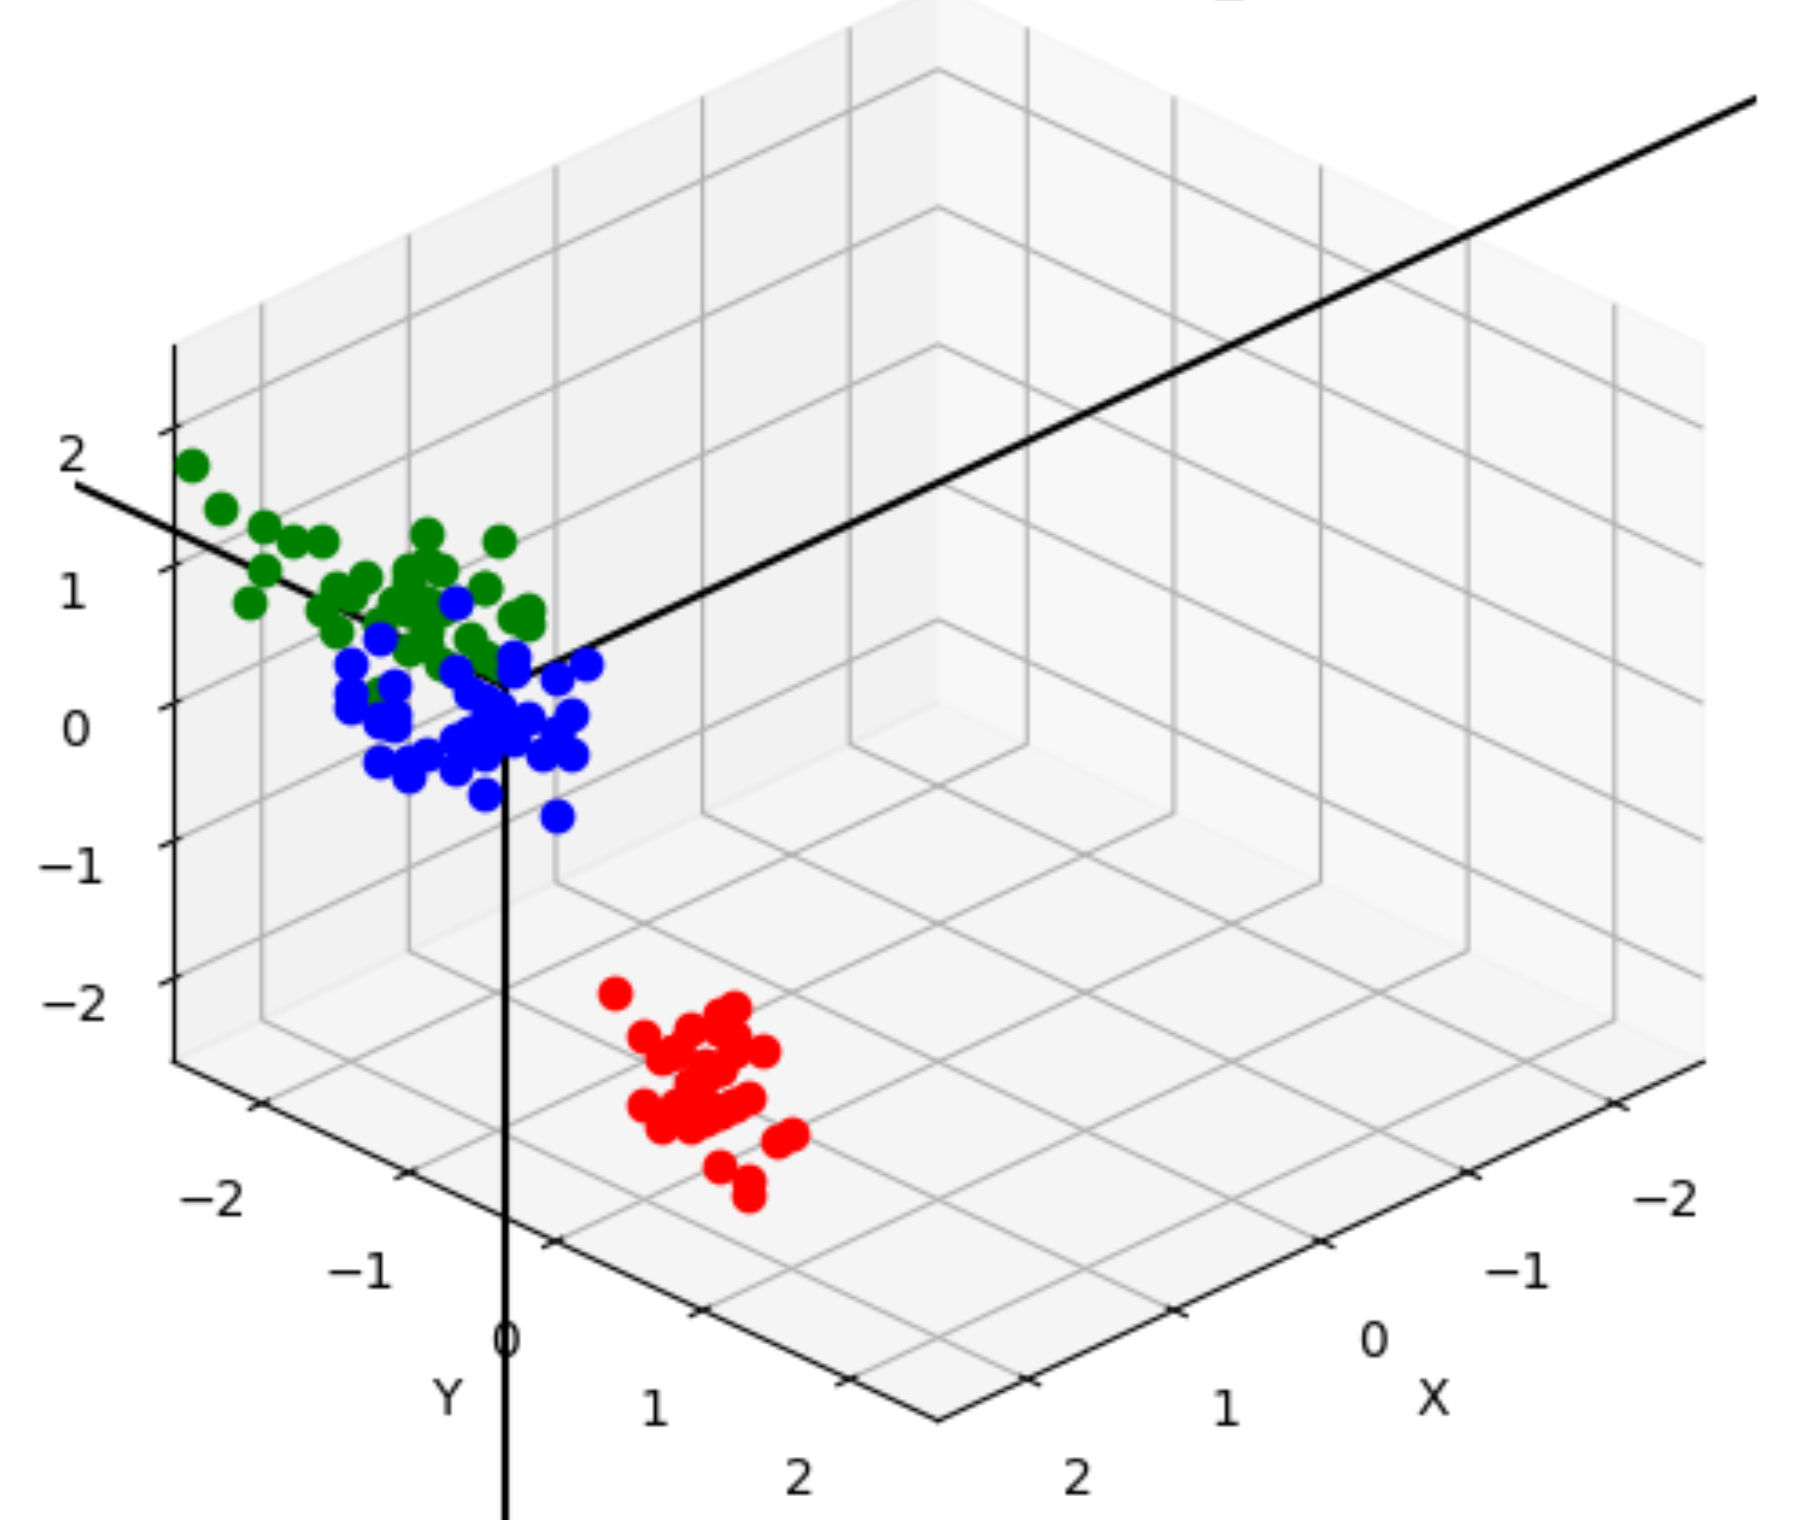
\includegraphics[width=0.7\linewidth]{fig/veronese_A1.png}
        \caption{$\mathcal{A}_1$ doesn't separate blue class well}
        \label{fig:veronese_A1}
    \end{subfigure}
    \\ % Creates a new line for the next subfigures
    
    \begin{subfigure}{0.45\textwidth}
        \centering
        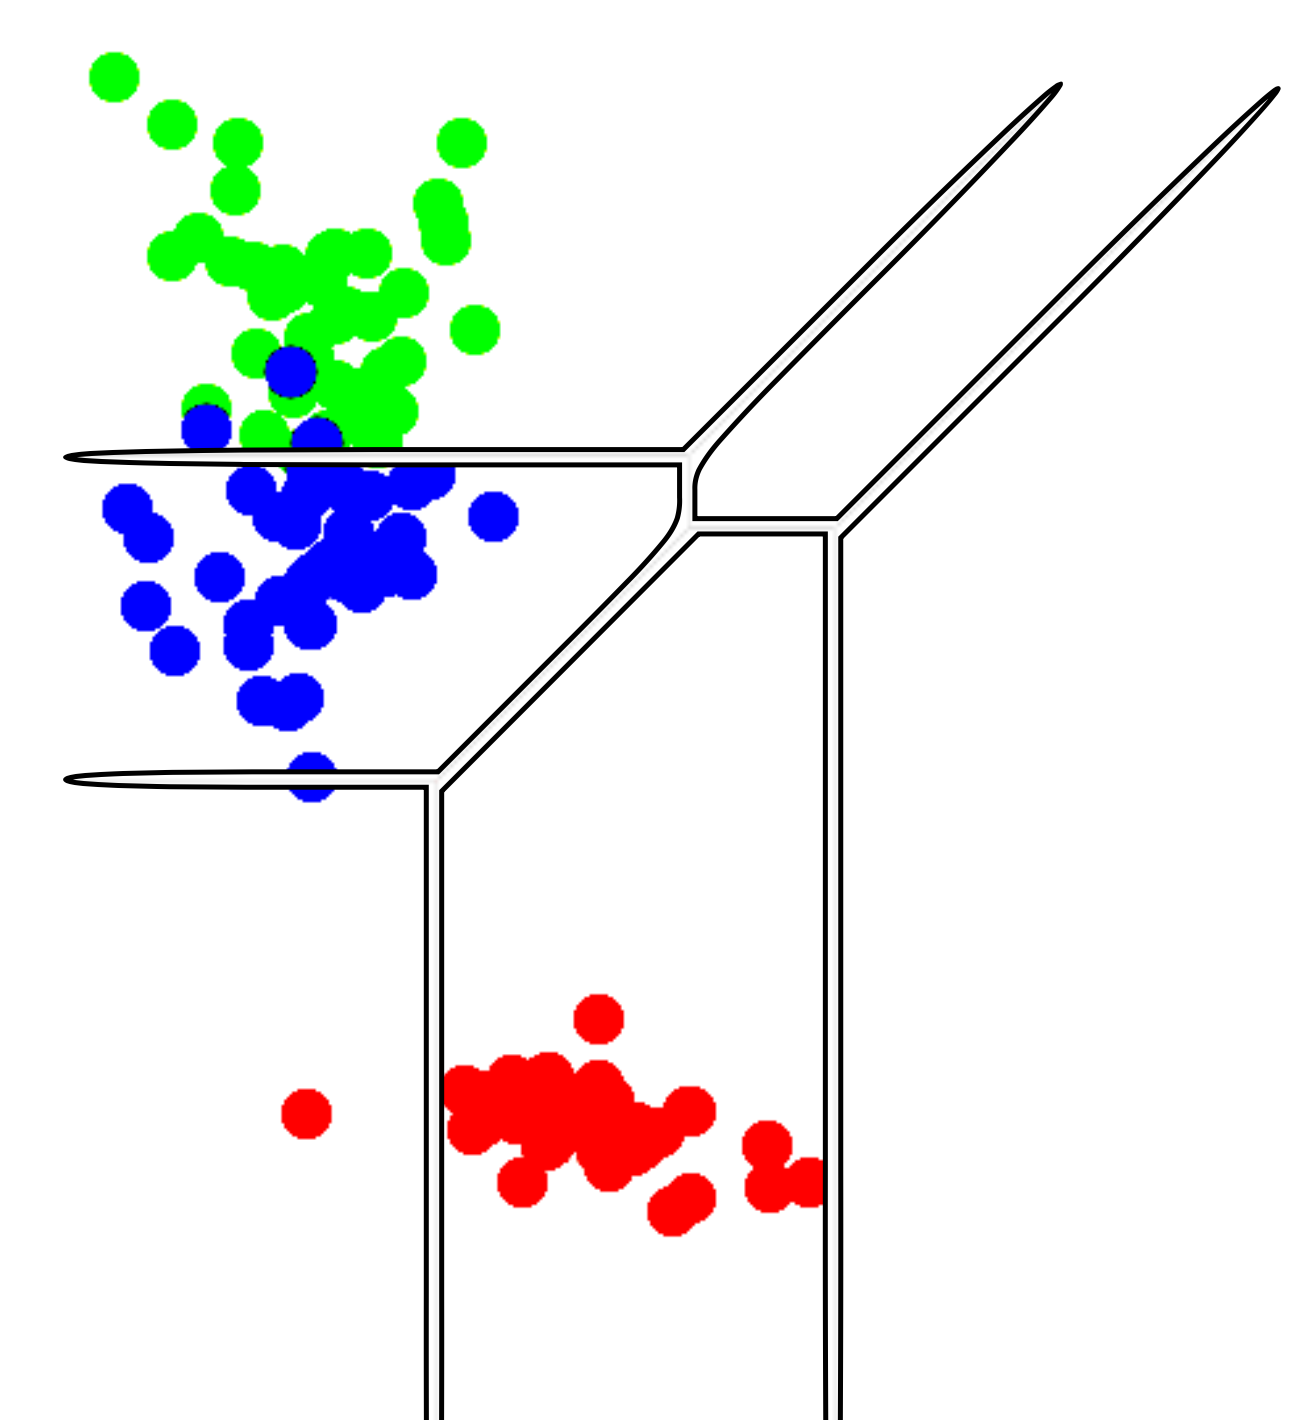
\includegraphics[width=\linewidth]{fig/veronese_A2.png}
        \caption{$\mathcal{A}_2$ is way better}
        \label{fig:veronese_A2}
    \end{subfigure}
    \hfill % Adds horizontal space between the subfigures
    \begin{subfigure}{0.45\textwidth}
        \centering
        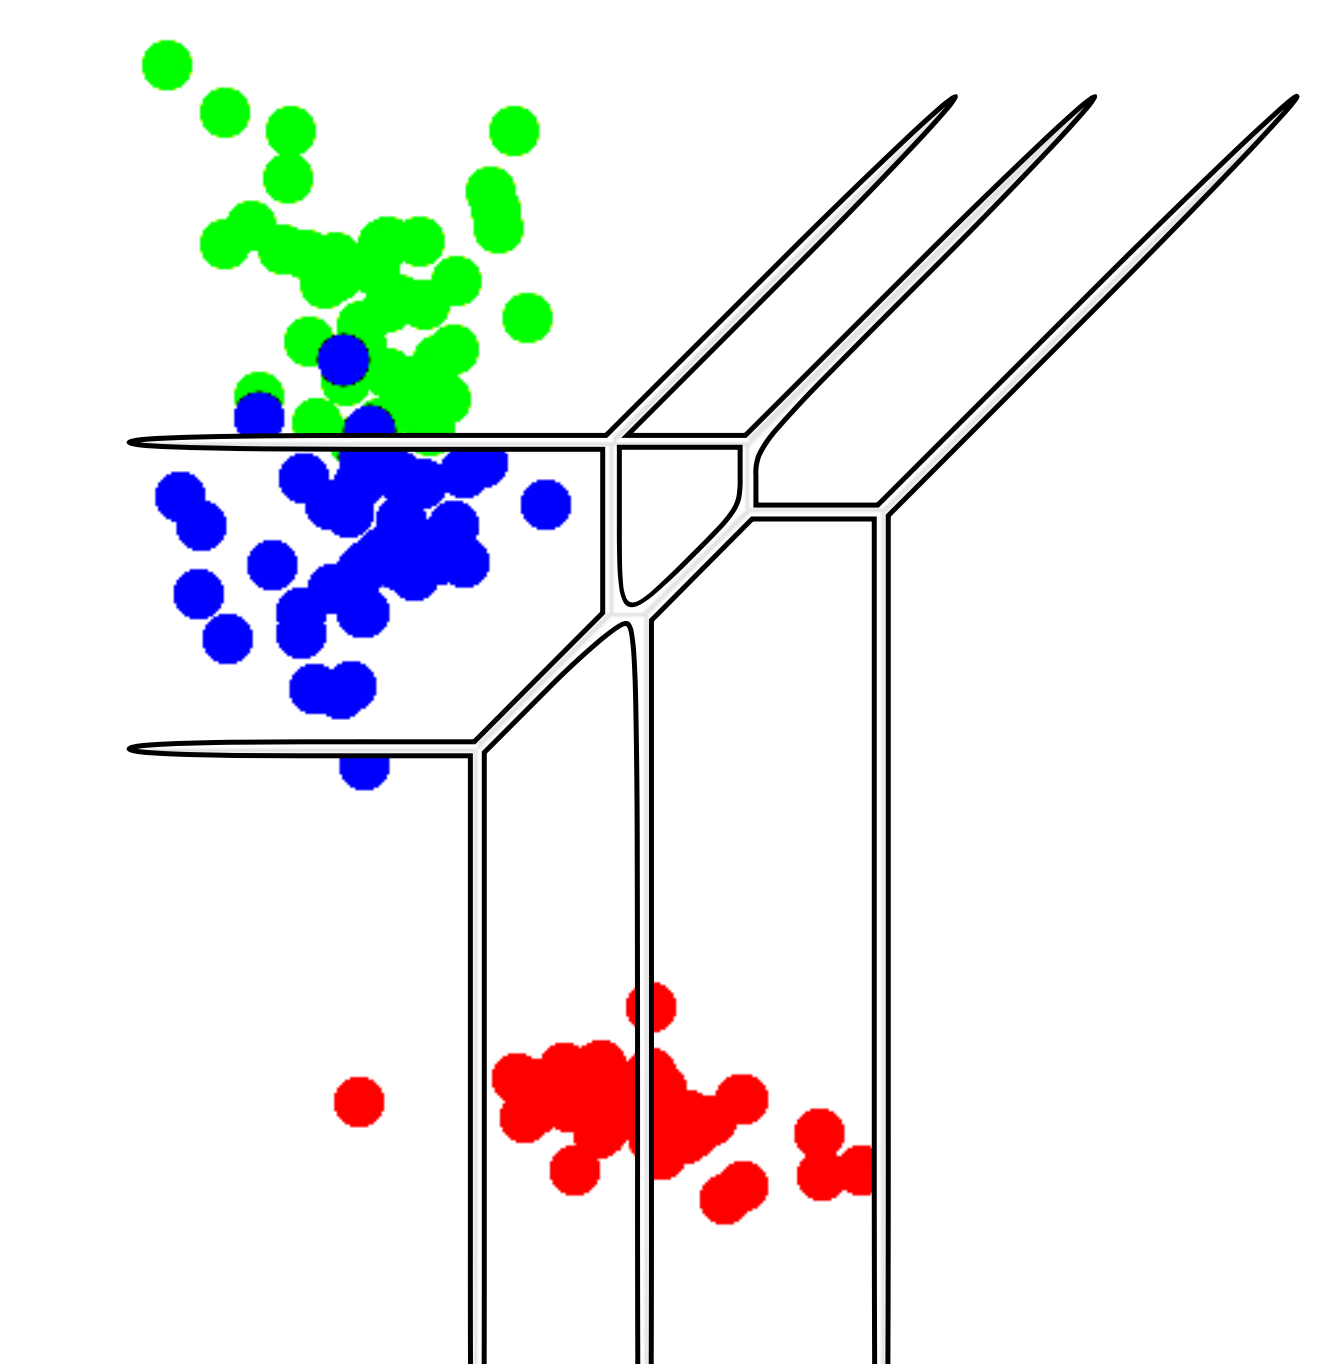
\includegraphics[width=\linewidth]{fig/veronese_A3.png}
        \caption{$\mathcal{A}_3$ overfits data}
        \label{fig:veronese_A3}
    \end{subfigure}

    \caption{Decision boundaries for $s\in\{1,2,3\}$}
    \label{fig:decision_boundaries}
\end{figure}

\begin{example}
In Figure \ref{fig:decision_boundaries}, we visualize the decision boundaries of the Iris classifier depending on scale parameter $s$. We remove the last feature of this dataset to have visualizable, 3-dimensional data.

For the last two figures, the tropical polynomial represented was rendered with Polymake, and the overlay with the data points was done by hand in an approximate - but very representative - manner.
\end{example}

\subsection{Linear Hyperplanes Look Tropical on Log Paper}

Let $X_{ij}$ be our point clouds, and for $\beta>0$, let's define
$x^{\beta}=(x_{ij}^{\beta}:=e^{\beta X_{ij}})_{ij}$. We will show
that separating different classes from $x^{\beta}$ using a linear
SVM, when $\beta$ tends toward infinity, yields a separating hyperplane
that converges towards a tropical hyperplane in the initial space.

Our method, by directly outputting an optimal-margin separating tropical
hyperplane in pseudo-polynomial time, is expected to achieve better
results. If $\beta$ is small, we might indeed be far away from the
limiting tropical hypersurface; conversely, as $\beta$ approaches
infinity, numerical error becomes predominant.

\begin{figure}[h]
\centering \includegraphics[scale=0.1]{\string"fig/linear log-exp kernel\string".png}
\includegraphics[scale=0.1]{\string"fig/tropical svm\string".png} 
\end{figure}


\subsubsection{Tropical hyperplanes are limiting classical hyperplanes}

Under the assumption that the $x_{ij}^{\beta}$ are linearly separable
\textbf{\emph{(strong assumption because it has to hold for all values
of $\beta$)}}, we compute a support vector classifier without intercept
term, whose separation surface's equation is: 
\[
H^{\beta}:\quad w^{\beta}\cdot x=0,
\]
where all positive (resp. negative) points verify $w^{\beta}\cdot x\ge1$
(resp. $w^{\beta}\cdot x\le-1$). We write 
\[
w_{i}^{\beta}=\sigma_{i}e^{\beta W_{i}^{\beta}},
\]
where $\sigma_{i}\in\{\pm1\}$ and $W_{i}^{\beta}\in\mathbb{R}\cup\{-\infty\}$.
For now, we simplify the study by considering a fixed $W_{i}$ value
and $w_{i}^{\beta}=\sigma_{i}e^{\beta W_{i}}$. 
\begin{lem}
(Maslov's sandwich) For $\beta>0$ and $I\subset[d]$ we have: 
\[
0\leq\beta^{-1}\log\left(\sum_{i\in I}e^{\beta(W_{i}+X_{ij})}\right)-\max_{i\in I}(W_{i}+X_{ij})\le\beta^{-1}\log d.
\]
\end{lem}

\begin{proof}
Let $\beta>0$ and $I\subset[d]$. We have: 
\[
\exp\left\{ \beta\max_{i\in I}\left(W_{i}+X_{ij}\right)\right\} \le\sum_{i\in I}e^{\beta(W_{i}+X_{ij})}\le d\cdot\exp\left\{ \beta\max_{i\in I}\left(W_{i}+X_{ij}\right)\right\} ,
\]
hence the result by taking the logarithm and dividing by $\beta$. 
\end{proof}
\begin{prop}
Defining $H^{\text{trop}}$ as the hyperplane of apex $(-W_{i})_{i\in[d]}$,
signed using $I^{+}:=\{i\in[d],\quad\sigma_{i}>0\}$ and $I^{-}:=[d]\backslash I^{+}$,
we have: 
\[
d_{H}\left(\log H^{\beta},H^{\text{trop}}\right)\le\beta^{-1}\log d,
\]
where $d_{H}$ is the tropical Haussdorf distance. Hence $\log H^{\beta}\longrightarrow H^{\text{trop}}$
as $\beta\longrightarrow+\infty$. 
\end{prop}

\begin{proof}
Let $\beta>0$ and $X\in H^{\beta}$. By writing the inequalities
from previous lemma with $I^{+}$ and $I^{-}$, and as $$\beta^{-1}\log\left(\sum_{i\in I^{+}}e^{\beta(W_{i}+X_{ij})}\right)=\beta^{-1}\log\left(\sum_{i\in I^{-}}e^{\beta(W_{i}+X_{ij})}\right),$$
substracting the first to second inequality yields: 
\[
-\beta^{-1}\log d\le\max_{i\in I^{+}}(W_{i}+X_{ij})-\max_{i\in I^{-}}(W_{i}+X_{ij})\le\beta^{-1}\log d.
\]
hence $d(X,H^{\text{trop}})\le\beta^{-1}\log d$.

Reciprocally, let $Y\in H^{\text{trop}}$ and $X=Y+\delta\mathbf{1}_{I^{+}}$,
with $\delta$ to be defined later. To have $Y\in H^{\beta}$, we
have to ensure that: 
\[
w^{\beta}\cdot y=0,
\]
which amounts to 
\[
\sum_{i\in[d]}\sigma_{i}e^{\beta W_{i}}e^{\beta X_{i}}=0.
\]
By separating the positive and negative terms, and taking the logarithm,
we get 
\[
\beta\delta+\log\left(\sum_{i\in I^{+}}e^{\beta(W_{i}+X_{ij})}\right)=\log\left(\sum_{i\in I^{-}}e^{\beta(W_{i}+X_{ij})}\right),
\]
which similarily yields 
\[
\delta\le\left|\beta^{-1}\log\left(\sum_{i\in I^{+}}e^{\beta(W_{i}+X_{ij})}\right)-\beta^{-1}\log\left(\sum_{i\in I^{-}}e^{\beta(W_{i}+X_{ij})}\right)\right|\le\beta^{-1}\log d,
\]
hence $d(Y,H^{\beta})\le\beta^{-1}\log d$. 
\end{proof}
\begin{rem}
We note $L$ the order of magnitude of our data points, and $B$ a
typical number at which the computer starts having numerical errors
or overflow (typically, for C integer calculations, $B=2^{16}-1)$.
We want to have $\beta L\ll\log B$ (that is, no numerical error),
and $\beta^{-1}\log d\ll L$ (good convergence towards tropical hyperplane),
i.e $d\ll B$. By directly computing logarithms, for instance, our
method should be very suitable for $d\apprge65535$ dimensions using
C integers. 
\end{rem}


\subsubsection{Finding tropical apex}

In the classical hard-margin setting, admissible $w$ vectors verify
$w^{T}x^{+}\ge1$ (resp. $w^{T}x^{-}\le-1$) for positive (resp. negative)
vectors. Thus they belong to the polytope $P^{\beta}$ where 
\[
P^{\beta}:=\left\{ w\in\mathbb{R}^{d},\quad w^{T}x_{j_{+}}^{\beta}\ge1\text{ and }w^{T}x_{j_{-}}^{\beta}\le-1,\forall j_{+},j_{-}\in J^{+},J^{-}\right\} .
\]

We hope that $L_{\sigma}(P^{\beta}):=\left\{ (\beta^{-1}\log(\sigma_{i}w_{i}))_{i\in[d]}\right\} $
converges towards the corresponding limiting tropical polytope $P_{\sigma}^{\text{trop}}:=P_{\sigma,+}^{\text{trop}}\cap P_{\sigma,-}^{\text{trop}}$,
where 
\[
P_{+,\sigma}^{\text{trop}}:=\left\{ W\in(\mathbb{R}\cup\{-\infty\})^{d},\quad\max_{i,\sigma_{i}=1}(W_{i}+X_{ij}^{\sigma})\ge\max_{i,\sigma_{i}=-1}(W_{i}+X_{ij}^{\sigma})\vee0,\forall j\in J^{+}\right\} .
\]
and 
\[
P_{-,\sigma}^{\text{trop}}:=\left\{ W\in(\mathbb{R}\cup\{-\infty\})^{d},\quad\max_{i,\sigma_{i}=-1}(W_{i}+X_{ij}^{\sigma})\le\max_{i,\sigma_{i}=1}(W_{i}+X_{ij}^{\sigma})\vee0,\forall j\in J^{-}\right\} .
\]

\begin{thm}
(Cite the corresponding article) When points $x_{ij}^{\beta}$ are
in a general position, \textbf{(clarify what this means as $\beta$}
\textbf{approaches infinity)} 
\[
\lim_{\beta\rightarrow+\infty}L_{\sigma}(P^{\beta})=P_{\sigma}^{\text{trop}},
\]
with respect to the Haussdorf distance. 
\end{thm}

We proved the convergence of the logarithm of linear hypersurfaces
towards a tropical limiting hypersurface, when the apex is fixed.
However, in practice, there is an underlying double limit here: for
each $\beta$ value, we compute an apex in the exponentialized space
and we hope it will converge towards a fixed apex in the initial space:
let's consider $w_{i}^{\beta}=\sigma_{i}e^{\beta W_{i}^{\beta}}$
again. 
\begin{thm}
(Cite the corresponding article) 
\[
W^{\infty}:=\lim_{\beta\rightarrow+\infty}\beta^{-1}\log w^{\beta}\in\underset{W\in P^{\text{trop}}}{\arg\min}\left(\max w\right).
\]
\end{thm}


\subsubsection{Computing limiting margin (experimental)}

In the classical setting, the margin is $\lVert w\rVert^{-1}$, described
by the vector $w/\lVert w\rVert^{2}$. Conjecturing that this vector,
when mapped back to the initial space, gives a meaningful approximation
of the margin (prove it), we can compute the norm of this limiting
vector. For $\beta>0$: 
\begin{align*}
\beta^{-1}\log\left(\frac{w^{\beta}}{\lVert w^{\beta}\rVert^{2}}\right) & =\beta^{-1}\log w^{\beta}-2\log\lVert e^{\beta W^{\beta}}\rVert^{\beta^{-1}}.
\end{align*}
Where the term $\log\lVert e^{\beta W^{\beta}}\rVert^{\beta^{-1}}\rightarrow\max\left|w^{\beta}\right|$,
and $\beta^{-1}\log w^{\beta}\rightarrow W^{\infty}$. Hence: 
\[
\left\lVert \beta^{-1}\log\left(\frac{w^{\beta}}{\lVert w^{\beta}\rVert^{2}}\right)\right\rVert \longrightarrow\max W^{\infty}-\min W^{\infty}
\]
would give a good approximation of the limiting margin.

\newpage{} \bibliographystyle{plain}
\bibliography{ea}

\end{document}
